\documentclass[aspectratio=169]{beamer}
\usepackage{booktabs}
\usepackage{xcolor}
\usepackage{changepage}
\usepackage[export]{adjustbox}
\usepackage{booktabs}
\usepackage{graphbox}
\usepackage[absolute,overlay]{textpos}
\usepackage{minted}
\usepackage{mdframed}

\usetheme[numbering=fraction,progressbar=frametitle]{metropolis}


% Backup
\newcommand{\backupbegin}{
   \newcounter{finalframe}
   \setcounter{finalframe}{\value{framenumber}}
}
\newcommand{\backupend}{
   \setcounter{framenumber}{\value{finalframe}}
}


% Colors
\definecolor{myBlue}{RGB}{21, 56, 110}
\definecolor{myRed}{RGB}{174,0,34}
\definecolor{myRedBg}{RGB}{251, 217, 224}
\definecolor{greySAS}{RGB}{167,166,166}
\definecolor{greyCU}{RGB}{44,46,53}

\setbeamercolor{title}{fg=myBlue}
\setbeamercolor{background canvas}{bg=white}
\setbeamercolor{normal text}{fg=black}
\setbeamercolor{frametitle}{fg=myBlue, bg=white}
\setbeamercolor{section title}{fg=myBlue}
\setbeamercolor{title separator}{fg=myRed,bg=myRedBg}
\setbeamercolor{progress bar}{fg=myRed,bg=myRedBg}
\setbeamercolor{structure}{fg=myRed}


% Frame around codeblocks
\surroundwithmdframed{minted}


% Thicker progress bar
\makeatletter
\setlength{\metropolis@titleseparator@linewidth}{1pt}
\setlength{\metropolis@progressonsectionpage@linewidth}{1pt}
\setlength{\metropolis@progressinheadfoot@linewidth}{1pt}
\makeatother


% Commands
\newcommand{\bluetext}[1]{%
  \textcolor{myBlue}{#1}
}
\newcommand{\redtext}[1]{%
  \textcolor{myRed}{#1}
}


% Title
\title{PandoraPFA for FCC-ee LAr Calorimeter}
\author{Juraj~Smie\v{s}ko\inst{1,2}}
\institute{\inst{1} Charles University, Czechia \\
           \inst{2} Slovak Academy of Sciences, Slovakia}
\date{\footnotesize
      Noble Liquid Calorimetry for Future Accelerator Experiments \\
      03 March 2022}

%
% -----------------------------------------------------------------------------
%
\begin{document}


{%
  \setbeamercolor{background canvas}{bg=greyCU}
  \begin{frame}[noframenumbering]
    \centering
    \vspace{1cm}
    
\includegraphics[width=.25\textwidth]{figures/CU_red_white_logo.pdf}
    \thispagestyle{empty}
  \end{frame}
}

\begin{frame}
  \titlepage{}
  \thispagestyle{empty}
\end{frame}

\begin{frame}
  \frametitle{\bf Particle Flow}

  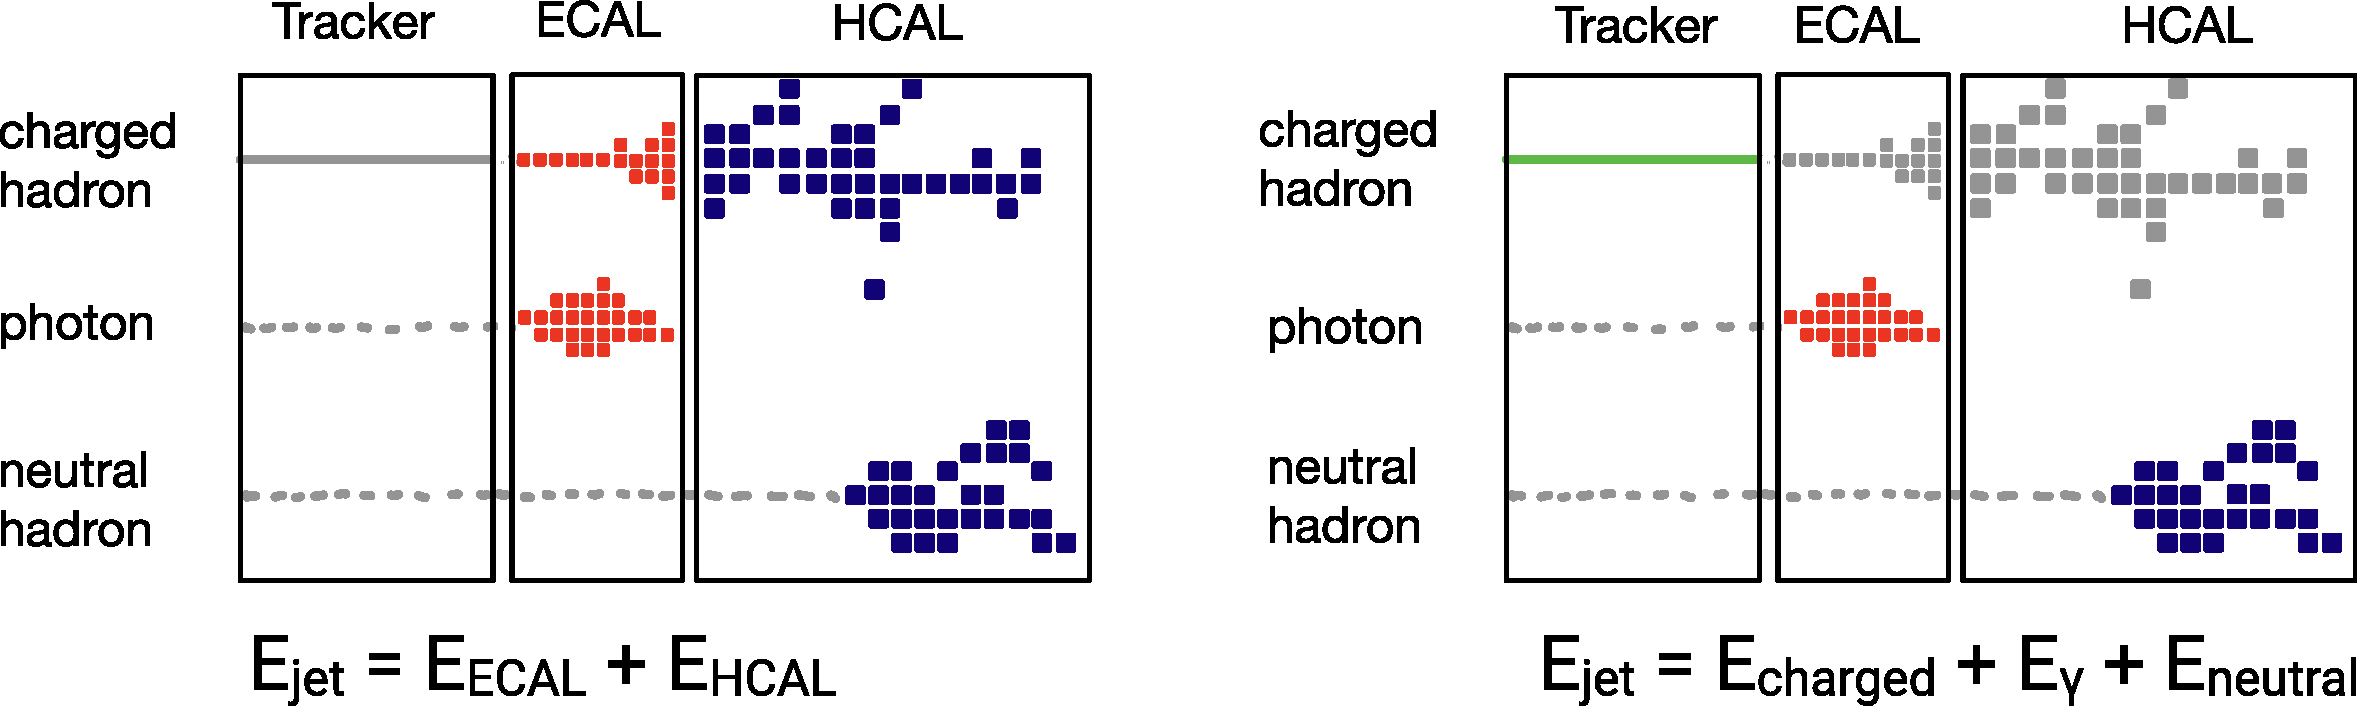
\includegraphics[width=\linewidth]{figures/particle_flow_diagram.pdf}
  \vspace{-1.5ex}
  \hspace{6.7em} 30\% + 70\% \hspace{14.5em} 60\% + 30\% + 10\%

  \begin{columns}[c]
    \column{.5\textwidth}
    \begin{itemize}
      \item Reconstruct every particle in the event with the best possible
            precision
      \item Combine the measurements in subdetectors in an optimal way
    \end{itemize}

    \column{.5\textwidth}
    \begin{itemize}
      \item Charged particles dominated by tracker
      \item Calorimetry mostly for neutral particles
      \item \bluetext{\bf Enemy: Confusion}
    \end{itemize}
  \end{columns}

  \begin{textblock*}{\paperwidth}(4pt, 0.15\textheight)
    \tiny
    \href{https://indico.cern.ch/event/932973/}
         {source}
  \end{textblock*}
\end{frame}


\begin{frame}[fragile]
  \frametitle{PandoraPFA I.}

  \begin{itemize}
    \item Framework which employs multitude of pattern recognition algorithms
      to \bluetext{\bf form/manipulate clusters} and \bluetext{\bf create PFOs}
      (particle flow objects)
    \item To facilitate different algorithms there are several layers
    \item The algorithms can be selected in a steering xml
  \end{itemize}


  \begin{columns}[c]
    \column{.55\textwidth}

    \begin{center}
      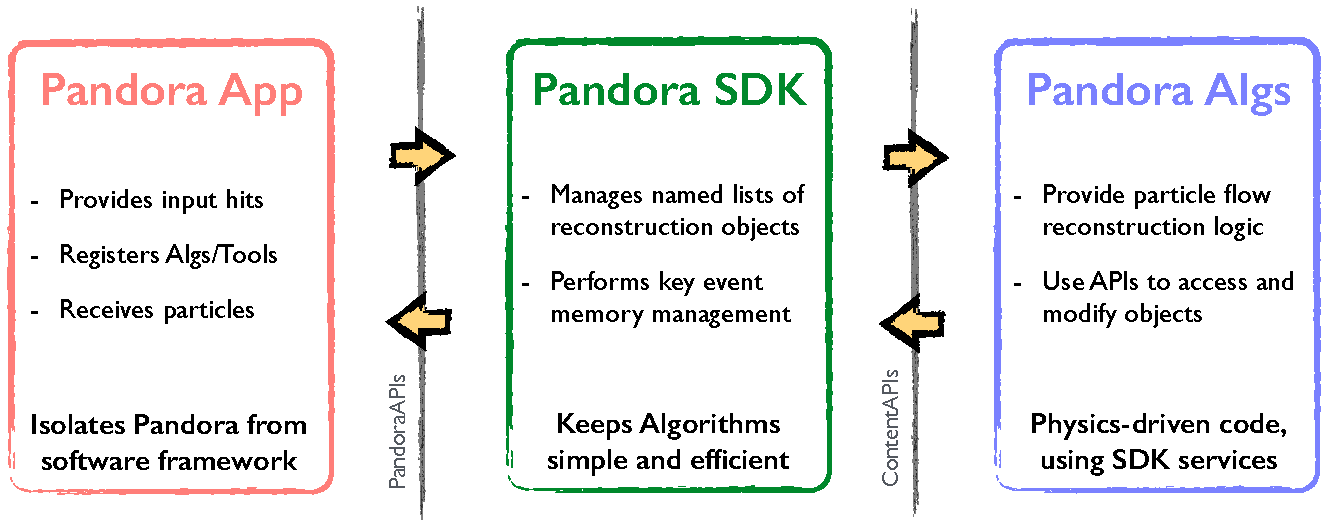
\includegraphics[width=\textwidth]{figures/pandora_apis.pdf}
    \end{center}

    \column{.45\textwidth}

    \fontsize{5}{8} \selectfont
    \begin{minted}{xml}
<algorithm type = "ConeClustering" instance = "Reclustering1">
    <TanConeAngleFine>0.24</TanConeAngleFine>
    <TanConeAngleCoarse>0.4</TanConeAngleCoarse>
    <AdditionalPadWidthsFine>2</AdditionalPadWidthsFine>
    <AdditionalPadWidthsCoarse>2</AdditionalPadWidthsCoarse>
    <SameLayerPadWidthsFine>2.24</SameLayerPadWidthsFine>
    <SameLayerPadWidthsCoarse>1.44</SameLayerPadWidthsCoarse>
    <MaxTrackSeedSeparation>100</MaxTrackSeedSeparation>
    <MaxLayersToTrackSeed>0</MaxLayersToTrackSeed>
    <MaxLayersToTrackLikeHit>0</MaxLayersToTrackLikeHit>
    <TrackPathWidth>0</TrackPathWidth>
</algorithm>
    \end{minted}
  \end{columns}


  \begin{textblock*}{\paperwidth}(4pt, 1.1\textheight)
    \tiny
    \href{https://github.com/PandoraPFA/Documentation/blob/master/Pandora_Example.pdf}
         {source}
  \end{textblock*}
\end{frame}


\begin{frame}
  \frametitle{PandoraPFA II.}

  \begin{center}
    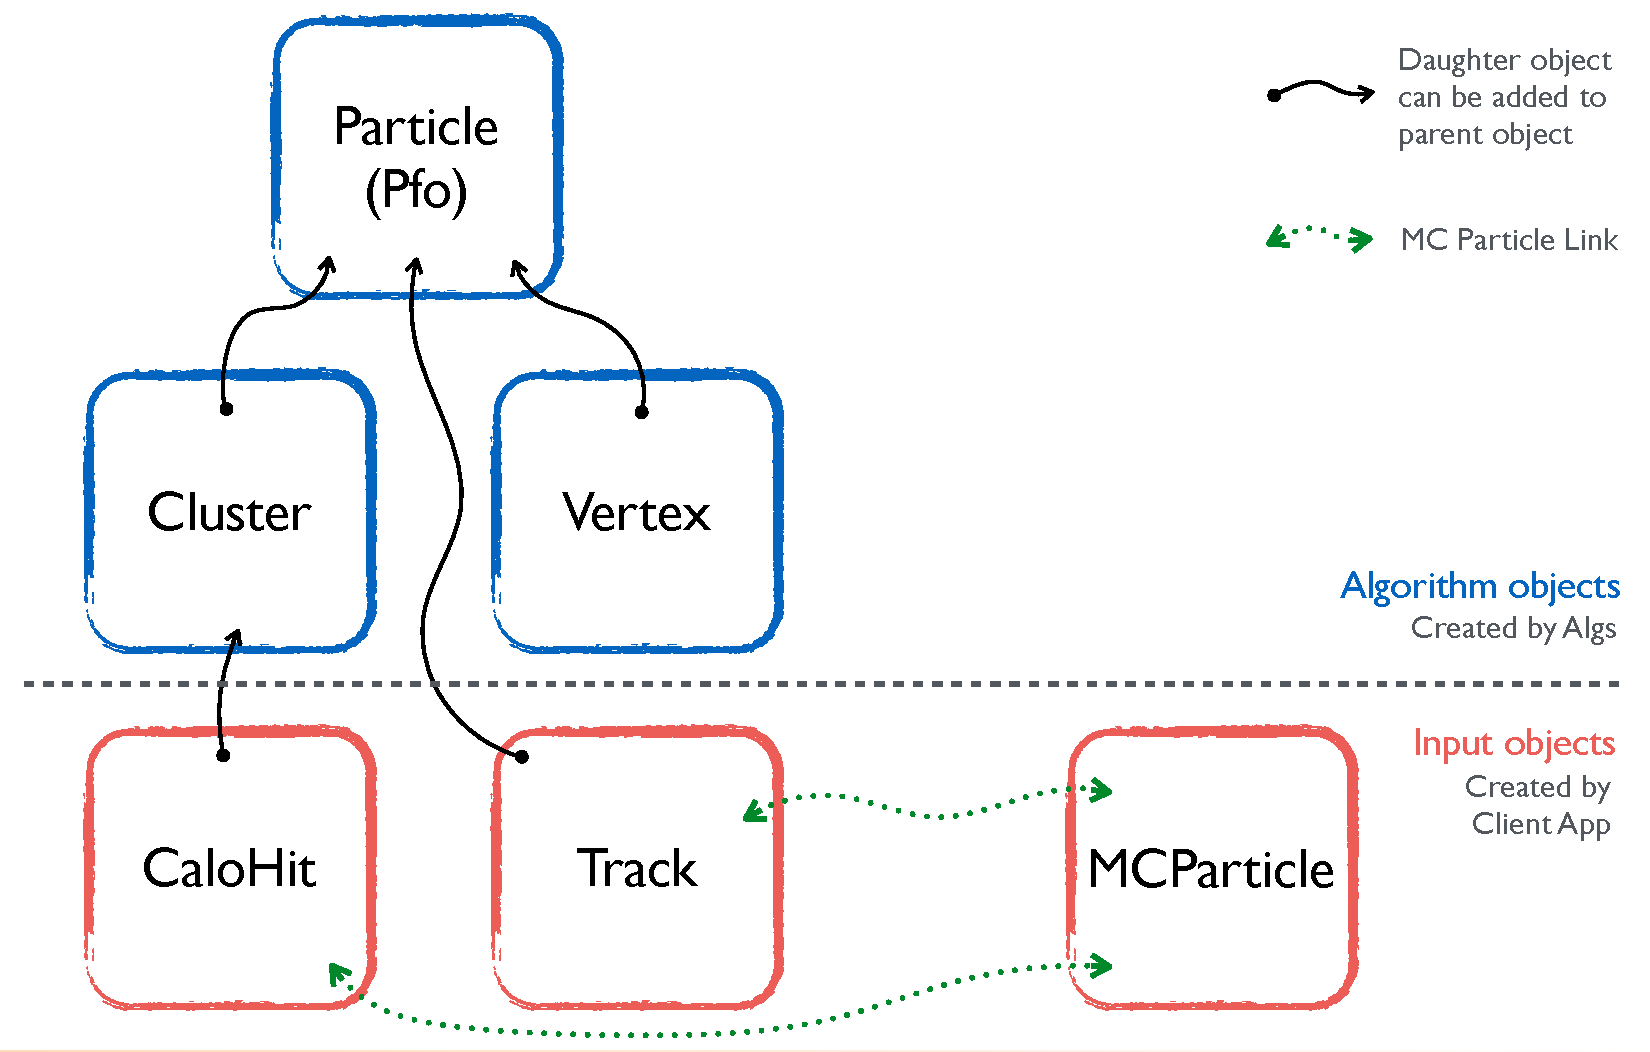
\includegraphics[width=.8\textwidth]{figures/pandora_edm.pdf}
  \end{center}

  \begin{textblock*}{\paperwidth}(4pt, 0.15\textheight)
    \tiny
    \href{https://github.com/PandoraPFA/Documentation/blob/master/Pandora_Example.pdf}
         {source}
  \end{textblock*}
\end{frame}


\begin{frame}
  \frametitle{Wrappers}

  \begin{columns}[c]
    \column{.5\textwidth}

    \bluetext{\bf DDMarlinPandora}

    \begin{itemize}
      \item Developed for ILC
      \item Pandora application wrapped inside Marlin processor
      \item Conversion between LCIO and Pandora datamodel
            \begin{itemize}
              \item CaloHits
              \item Tracks
              \item MCParticles
              \item Geometry
            \end{itemize}
      \item Provides xml settings file
    \end{itemize}

    \column{.5\textwidth}

    \bluetext{\bf k4MarlinWrapper}
    \begin{itemize}
      \item Wraps Marlin processor inside Gaudi algorithm
      \item Converts from EDM4hep datamodel into LCIO datamodel
      \item Marlin processor is steered by python script instead of xml file
    \end{itemize}
  \end{columns}


\end{frame}


\begin{frame}[fragile]
  \frametitle{The Plan for Running Pandora}

  \begin{center}
  \bluetext{\bf Run Pandora inside \texttt{DDMarlinPandora} inside
            \texttt{k4MarlinWrapper}}
  \end{center}

  \begin{columns}[c]
    \column{.55\textwidth}

    \begin{itemize}
      \item Considered to be \bluetext{\bf quickest} way to have Pandora running
      \item \redtext{\bf Disadvantage:} two datamodel conversions
      \item Over time, development of the native Key4hep wrapper
      \item \bluetext{\bf First step:} Get just Pandora clustering algorithm run
    \end{itemize}

    \column{.45\textwidth}

    \tiny
    \begin{minted}{python}
from Configurables import MarlinProcessorWrapper

pandora = MarlinProcessorWrapper('DDMarlinPandora')
pandora.OutputLevel = DEBUG
pandora.ProcessorType = 'DDPandoraPFANewProcessor'
pandora.Parameters = {
    'Verbosity': ['WARNING'],
    'PandoraSettingsXmlFile': ['/some/path'],
    'CreateGaps': [False],
    'ECalCaloHitCollections': ['ECalBarrelCells']
}
ApplicationMgr().TopAlg += [pandora]
\end{minted}
  \end{columns}
\end{frame}


\begin{frame}
  \frametitle{What is Missing?}

  \scriptsize
  PandoraPFA/\texttt{DDMarlinPandora} requires following components:

  \vspace{-1ex}

  \begin{itemize}\scriptsize
    \item \bluetext{Geometry description in DD4HEP format}
          \begin{itemize}\scriptsize
            \item IDEA-LAr already described in it, needs adjustments
          \end{itemize}
   \item \bluetext{Calorimeter hits}
          \begin{itemize}\scriptsize
            \item Conversions provided by
                  \texttt{DDMarlinPandora}/\texttt{k4MarlinWrapper}
          \end{itemize}
          % \begin{itemize}
          %   \item Conversion from LCIO datamodel to Pandora datamodel provided
          %         by \texttt{DDMarlinPandora} wrapper
          %   \item Conversion from EDM4hep datamodel provided by
          %         \texttt{k4MarlinWrapper}
          % \end{itemize}
    \item \redtext{Tracks alongside with vertexes}
          \begin{itemize}\scriptsize
            \item Requires custom code, base class provided
            % \item 
          \end{itemize}
    \item \bluetext{MCParticles}
          \begin{itemize}\scriptsize
            \item Conversions provided by
                  \texttt{DDMarlinPandora}/\texttt{k4MarlinWrapper}
          \end{itemize}
  \end{itemize}

  Also required are:

  \vspace{-1ex}

  \begin{itemize}\scriptsize
      \item Conversion of PFOs from Pandora datamodel
          \begin{itemize}\setlength{\itemsep}{.5ex}\scriptsize
            \item Conversions provided by
                  \texttt{DDMarlinPandora}/\texttt{k4MarlinWrapper}
          \end{itemize}
      \item Calibration of the calorimeter clusters
      \item Review of CLIC and ILD specific code
      \item Optimization of the algorithms
  \end{itemize}
\end{frame}


%
% -----------------------------------------------------------------------------
%
% \appendix
% \backupbegin{}
%
% \begin{frame}[c]
%   \begin{center}
%     \redtext{\Huge Backup}
%   \end{center}
% \end{frame}
%
%
%\backupend{}

\end{document}
